\documentclass{article}

\usepackage{fancyhdr}
\usepackage[dvipsnames]{xcolor}
\usepackage{extramarks}
\usepackage{amsmath}
\usepackage{amsthm}
\usepackage{amsfonts}
\usepackage{tikz}
\usepackage[plain]{algorithm}
\usepackage{algpseudocode}
\usepackage[shortlabels]{enumitem}
\usepackage{mathtools}
\usepackage{amssymb}
\usepackage{hyperref}
\usepackage{tikz}
\usepackage{pgfplots}

\usetikzlibrary{automata,positioning}

%
% Basic Document Settings
%

\topmargin=-0.45in
\evensidemargin=0in
\oddsidemargin=0in
\textwidth=6.5in
\textheight=9.0in
\headsep=0.25in

\linespread{1.1}

\pagestyle{fancy}
\lhead{\hmwkAuthorName}
\chead{\hmwkClassTime (\hmwkClassInstructor): \hmwkTitle}
\lfoot{\lastxmark}
\cfoot{\thepage}

\renewcommand\headrulewidth{0.4pt}
\renewcommand\footrulewidth{0.4pt}

\setlength\parindent{0pt}

%
% Create Problem Sections
%

\newcommand{\enterProblemHeader}[1]{
    \nobreak\extramarks{}{Problem \arabic{#1} continued on next page\ldots}\nobreak{}
    \nobreak\extramarks{Problem \arabic{#1} (continued)}{Problem \arabic{#1} continued on next page\ldots}\nobreak{}
}

\newcommand{\exitProblemHeader}[1]{
    \nobreak\extramarks{Problem \arabic{#1} (continued)}{Problem \arabic{#1} continued on next page\ldots}\nobreak{}
    \stepcounter{#1}
    \nobreak\extramarks{Problem \arabic{#1}}{}\nobreak{}
}

\setcounter{secnumdepth}{0}
\newcounter{partCounter}
\newcounter{homeworkProblemCounter}
\setcounter{homeworkProblemCounter}{1}
\nobreak\extramarks{Problem \arabic{homeworkProblemCounter}}{}\nobreak{}

\newcommand{\hmwkTitle}{Problem Set 2}
\newcommand{\hmwkDueDate}{February 16, 2024}
\newcommand{\hmwkClass}{Introduction to Economics}
\newcommand{\hmwkClassTime}{ECON 101}
\newcommand{\hmwkClassInstructor}{Robert McDonough}
\newcommand{\hmwkAuthorName}{\textbf{Rushil Umaretiya}}

%
% Title Page
%

\title{
    \vspace{2in}
    \textmd{\textbf{\hmwkClass:\ \hmwkTitle}}\\
    \normalsize\vspace{0.1in}\small{\textbf{Due\ on\ \hmwkDueDate\ at 11:59pm}}\\
    \normalsize\text{Tuesday/Thursday 3:30-4:45, Genome Sciences 100}\\
    \vspace{0.1in}\large{\textit{\hmwkClassInstructor\ - \hmwkClassTime}}
    \vspace{3in}
}

\author{\hmwkAuthorName\\\small{rumareti@unc.edu}}
\date{}

\renewcommand{\part}[1]{\textbf{\large Part \Alph{partCounter}}\stepcounter{partCounter}\\}

%
% Various Helper Commands
%

% Useful for algorithms
\newcommand{\alg}[1]{\textsc{\bfseries \footnotesize #1}}

% For derivatives
\newcommand{\deriv}[1]{\frac{\mathrm{d}}{\mathrm{d}x} (#1)}

% For partial derivatives
\newcommand{\pderiv}[2]{\frac{\partial}{\partial #1} (#2)}

% Integral dx
\newcommand{\dx}{\mathrm{d}x}

% Alias for the Solution section header
\newcommand{\solution}{\textbf{\large Solution}}

\newcommand{\question}[1]{\pagebreak\section{Question #1}}

% Probability commands: Expectation, Variance, Covariance, Bias
\newcommand{\E}{\mathrm{E}}
\newcommand{\Var}{\mathrm{Var}}
\newcommand{\Cov}{\mathrm{Cov}}
\newcommand{\Bias}{\mathrm{Bias}}

\begin{document}

\maketitle

\question{1}

Consider the daily market for a cup of coffee in Chapel Hill. Market demand for coffee is given by the equation \(P = 80 - \frac{1}{2}Q_d\), and market supply of coffee is given by \(P = 2 + \frac{Q_s}{37}\).
\begin{enumerate}[(a)]
    \item If the price of coffee is \$0, how many cups would sellers want to
    sell?
    \begin{align*}
        0 &= 2 + \frac{Q_s}{37}\\
        -2 &= \frac{Q_s}{37}\\
        Q_s &= -74\\
        Q_s &\approx 0
    \end{align*}

    If the price of coffee is \$0, sellers wouldn't want to sell any coffee.
    \item Calculate the equilibrium price of coffee and the quantity of coffee
    cups sold in Chapel Hill every day.
    \begin{align*}
        Q_s &= 37P - 74\\
        Q_d &= 160 - 2P\\
        37P - 74 &= 160 - 2P\\
        39P &= 234\\
        P &= 6\\
        Q &= 160 - 2(6)\\
        Q &= 148
    \end{align*}
    The equilibrium price of coffee is \$6, and the equilibrium quantity of coffee cups sold in Chapel Hill every day is 148.
    \item Draw a properly labeled diagram for the market for coffee in Chapel Hill.
    
    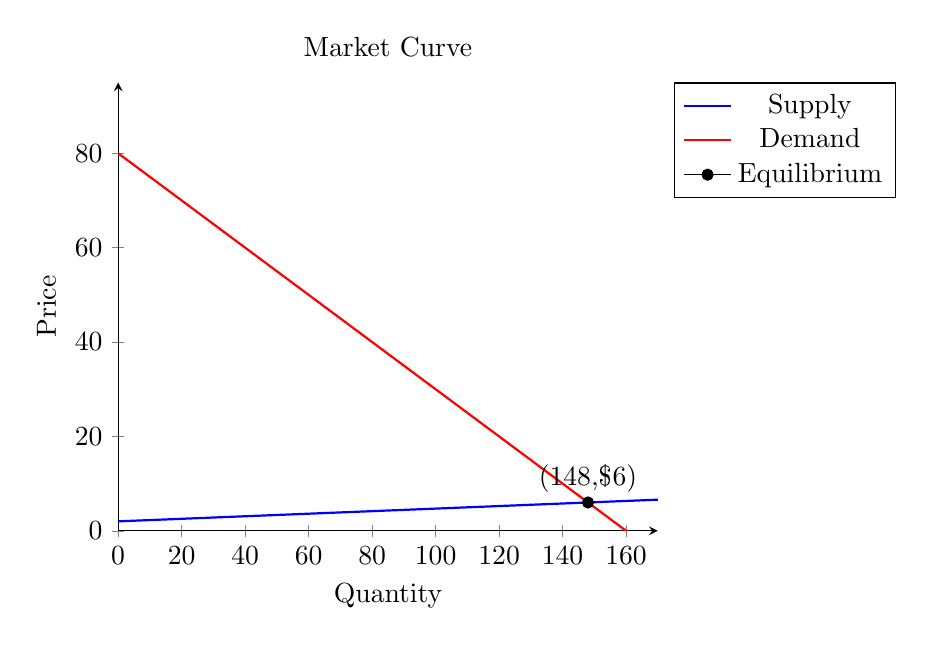
\begin{tikzpicture}
        \begin{axis}[
            title={Market Curve},
            ylabel={Price},
            xlabel={Quantity},
            xmin=0, xmax=170,
            ymin=0, ymax=95,
            axis lines=left,
            grid=none,
            legend pos=outer north east,
        ]

        \addplot[domain=0:200, color=blue, thick] {2 + x/37};
        \addlegendentry{Supply}

        \addplot[domain=0:200, color=red, thick] {80 - 0.5*x};
        \addlegendentry{Demand}
        

        \addplot[mark=*, color=black] coordinates {(148,6)} node[above] {(148,\$6)};
        \addlegendentry{Equilibrium}
        \end{axis}
    \end{tikzpicture}
    \pagebreak
    \item Use the midpoint formula to calculate the price elasticity of demand for coffee if the price of a cup of coffee changes from \$4 to \$5.
    
    At a price of \$4, the quantity demanded is 152. At a price of \$5, the quantity demanded is 150. Using the midpoint formula:
    \begin{align*}
        \text{Price Elasticity of Demand} &= \frac{\text{Percentage Change in Quantity Demanded}}{\text{Percentage Change in Price}}\\
        \text{Percentage Change in Quantity Demanded} &= \frac{150 - 152}{(150+152)/2} = -\frac{2}{151} = -0.013\\
        \text{Percentage Change in Price} &= \frac{5 - 4}{(5 + 4)/2} = \frac{1}{4.5} = 0.222\\
        \text{Price Elasticity of Demand} &= \frac{-0.078}{0.222} = -0.0596
    \end{align*}
    \item Use the midpoint formula to calculate the price elasticity of supply for coffee if the price of a cup of coffee changes from \$4 to \$5.
    
    At a price of \$4, the quantity supplied is 74. At a price of \$5, the quantity supplied is 111. Using the midpoint formula:
    \begin{align*}
        \text{Price Elasticity of Supply} &= \frac{\text{Percentage Change in Quantity Supplied}}{\text{Percentage Change in Price}}\\
        \text{Percentage Change in Quantity Supplied} &= \frac{111 - 74}{(111+74)/2} = \frac{37}{92.5} = 0.4\\
        \text{Percentage Change in Price} &= \frac{5 - 4}{(5 + 4)/2} = \frac{1}{4.5} = 0.222\\
        \text{Price Elasticity of Supply} &= \frac{0.4}{0.222} = 1.8
    \end{align*}
    \item Imagine that two new coffee shops open in Chapel Hill. Graph how this will impact the market for cups of coffee. Be sure to clearly indicate the direction in which price and quantity have moved if equilibrium has changed.
    
    This will cause the supply curve to shift to the right (down), as there will be more coffee available in the market. This will cause the equilibrium price to fall, and the equilibrium quantity to rise.

    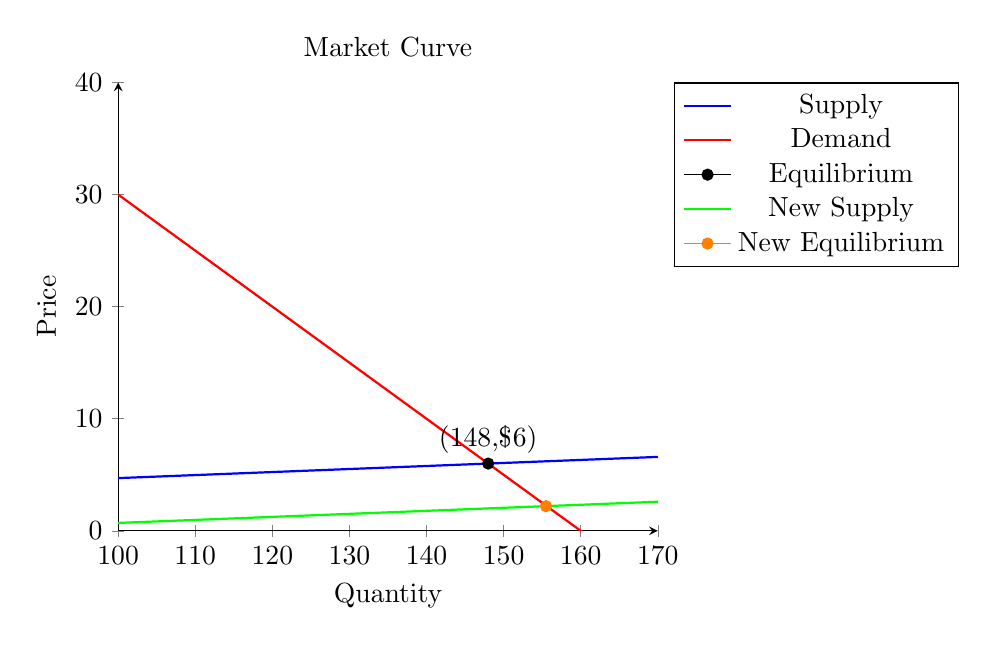
\begin{tikzpicture}
        \begin{axis}[
            title={Market Curve},
            ylabel={Price},
            xlabel={Quantity},
            xmin=100, xmax=170,
            ymin=0, ymax=40,
            axis lines=left,
            grid=none,
            legend pos=outer north east,
        ]

        \addplot[domain=0:200, color=blue, thick] {2 + x/37};
        \addlegendentry{Supply}

        \addplot[domain=0:200, color=red, thick] {80 - 0.5*x};
        \addlegendentry{Demand}
        
        \addplot[mark=*, color=black] coordinates {(148,6)} node[above] {(148,\$6)};
        \addlegendentry{Equilibrium}
        \addplot[domain=0:200, color=green, thick] {2 + x/37 -4};
        \addlegendentry{New Supply}

        \addplot[mark=*, color=orange] coordinates {(155.5,2.2)};
        \addlegendentry{New Equilibrium}
        \end{axis}
    \end{tikzpicture}
\end{enumerate}

\pagebreak

\question{2}

Economists have been interested in markets for illegal and addictive goods for a long time. One question that many economists have asked is whether \textcolor{OliveGreen}{marijuana} and alcohol are substitutes or complements. After North Carolina legalized \textcolor{OliveGreen}{marijuana}, Ben began to collect data on the alcohol and \textcolor{OliveGreen}{marijuana} markets to try to answer this question. He found that in August of 2019, the price of an ounce of \textcolor{OliveGreen}{marijuana} fell by 5\%, and that alcohol sales rose by 7\% directly afterwards.

\begin{enumerate}[(a)]
    \item Calculate the \textcolor{OliveGreen}{marijuana} cross-price elasticity of demand for alcohol.
    \begin{align*}
        \text{Cross-Price Elasticity of Demand} &= \frac{\text{Percentage Change in Quantity Demanded of Alcohol}}{\text{Percentage Change in Price of \textcolor{OliveGreen}{marijuana}}}\\
         &= \frac{0.07}{-0.05} = -1.4
    \end{align*}
    \item What does Ben's data indicate about the relationship between alcohol and \textcolor{OliveGreen}{marijuana}?
    
    Ben's data indicates that alcohol and \textcolor{OliveGreen}{marijuana} are complements, as the cross-price elasticity of demand is negative, which means as the price of \textcolor{OliveGreen}{marijuana} falls, and quantity demanded of \textcolor{OliveGreen}{marijuana} rises, the quantity demanded of alcohol also rises.
\end{enumerate}

\pagebreak

\question{3}

Consider the market for laptops during 2020, after the COVID pandemic began. For each of the following scenarios, graph how supply and/or demand will shift, and indicate how this will impact the equilibrium price and quantity of laptops sold in the U.S.

\begin{enumerate}[(a)]
    \item The government provides most U.S. adults with a \$1,200 stimulus check.
    
    Since the government is providing most U.S. adults with a \$1,200 stimulus check, this will cause the demand curve to shift to the right (up), as people will have more money to spend on laptops. This will cause the equilibrium price to rise, and the equilibrium quantity to rise.

    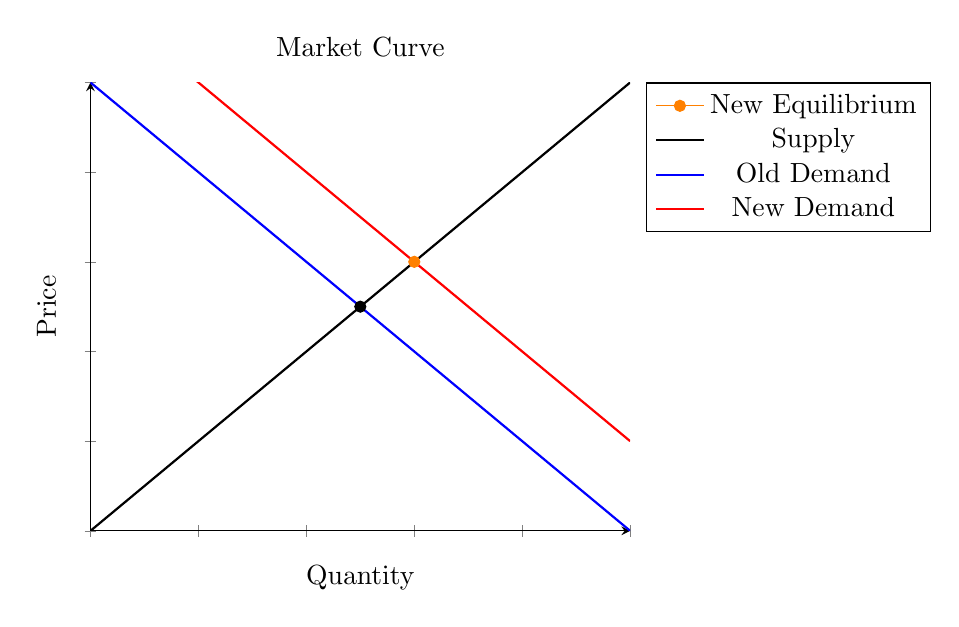
\begin{tikzpicture}
        \begin{axis}[
            title={Market Curve},
            ylabel={Price},
            xlabel={Quantity},
            yticklabel=\empty,
            xticklabel=\empty,
            xmin=0, xmax=10,
            ymin=0, ymax=10,
            axis lines=left,
            grid=none,
            legend pos=outer north east,
        ]
        

        \addplot[mark=*, color=orange] coordinates {(6,6)};
        \addlegendentry{New Equilibrium}


        \addplot[domain=0:10, color=black, thick] {x};
        \addlegendentry{Supply}
        
        \addplot[domain=0:10, color=blue, thick] {-x+10};
        \addlegendentry{Old Demand}

        \addplot[domain=0:10, color=red, thick] {-x+12};
        \addlegendentry{New Demand}

        \addplot[mark=*] coordinates {(5,5)};

        \end{axis}
    \end{tikzpicture}


    \item A global semiconductor shortage causes the price of semiconductors, a crucial component used in laptops, to rise dramatically.
    

    Since we see a rise in the price of semiconductors, this will cause the supply curve to shift to the left (up), as the cost of production for laptops will rise. This will cause the equilibrium price to rise, and the equilibrium quantity to fall.

    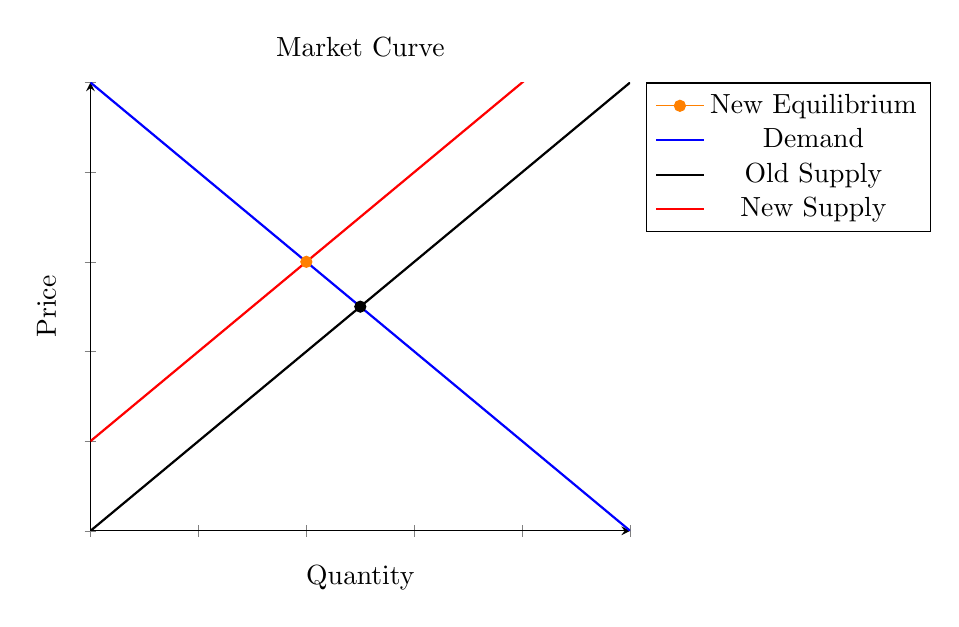
\begin{tikzpicture}
        \begin{axis}[
            title={Market Curve},
            ylabel={Price},
            xlabel={Quantity},
            yticklabel=\empty,
            xticklabel=\empty,
            xmin=0, xmax=10,
            ymin=0, ymax=10,
            axis lines=left,
            grid=none,
            legend pos=outer north east,
        ]
        

        \addplot[mark=*, color=orange] coordinates {(4,6)};
        \addlegendentry{New Equilibrium}

        \addplot[domain=0:10, color=blue, thick] {-x+10};
        \addlegendentry{Demand}

        \addplot[domain=0:10, color=black, thick] {x};
        \addlegendentry{Old Supply}

        \addplot[domain=0:10, color=red, thick] {x+2};
        \addlegendentry{New Supply}

        \addplot[mark=*] coordinates {(5,5)};
        
        \end{axis}
    \end{tikzpicture}
    \item The government provides most U.S. adults with a \$1,200 stimulus check. At the same time, a global semiconductor shortage causes the price of semiconductors, a crucial component used in laptops, to rise dramatically.
    
    Since both events are occurring at the same time, the demand curve will shift to the right (up) due to the stimulus check, and the supply curve will shift to the left (up) due to the rise in the price of semiconductors. This will cause the equilibrium price to rise, and an ambiguous effect on the equilibrium quantity.

    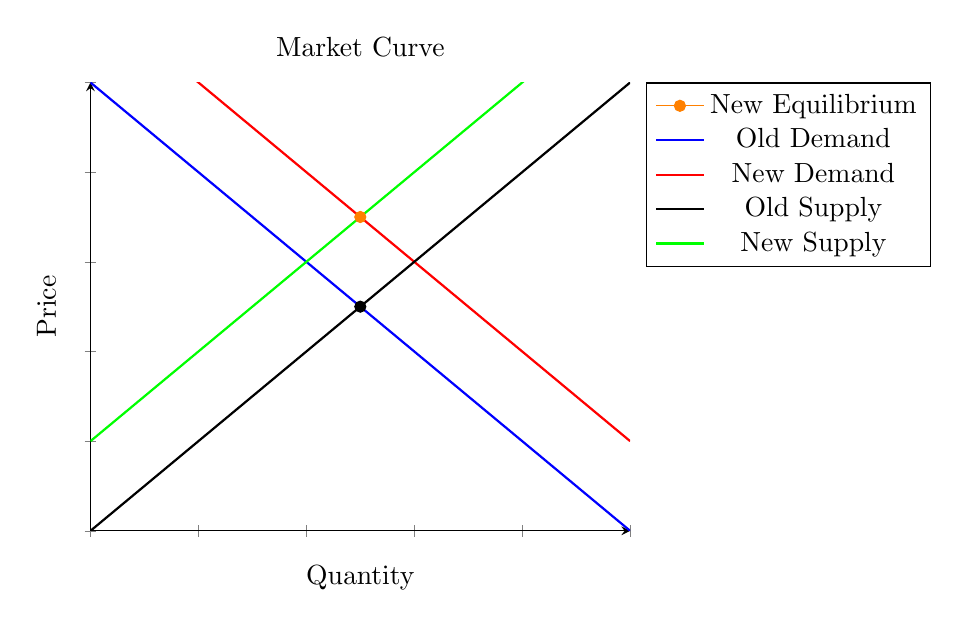
\begin{tikzpicture}
        \begin{axis}[
            title={Market Curve},
            ylabel={Price},
            xlabel={Quantity},
            yticklabel=\empty,
            xticklabel=\empty,
            xmin=0, xmax=10,
            ymin=0, ymax=10,
            axis lines=left,
            grid=none,
            legend pos=outer north east,
        ]
        

        \addplot[mark=*, color=orange] coordinates {(5,7)};
        \addlegendentry{New Equilibrium}

        \addplot[domain=0:10, color=blue, thick] {-x+10};
        \addlegendentry{Old Demand}

        \addplot[domain=0:10, color=red, thick] {-x+12};
        \addlegendentry{New Demand}

        \addplot[domain=0:10, color=black, thick] {x};
        \addlegendentry{Old Supply}

        \addplot[domain=0:10, color=green, thick] {x+2};
        \addlegendentry{New Supply}

        \addplot[mark=*] coordinates {(5,5)};
        
        \end{axis}
    \end{tikzpicture}

    \item A large percentage of the U.S. workforce begins to work from home for the duration of the pandemic. At the same time, laptop companies develop new software that lets the machines in their factories make twice as many laptops in a day.
    
    Since a large percentage of the U.S. workforce begins to work from home, this will cause the demand curve to shift to the right (up), as people will need laptops to work from home. At the same time, the supply curve will shift to the right (down), as the cost of production for laptops will fall. This will cause the equilibrium quantity to rise, and an ambiguous effect on the equilibrium price.

    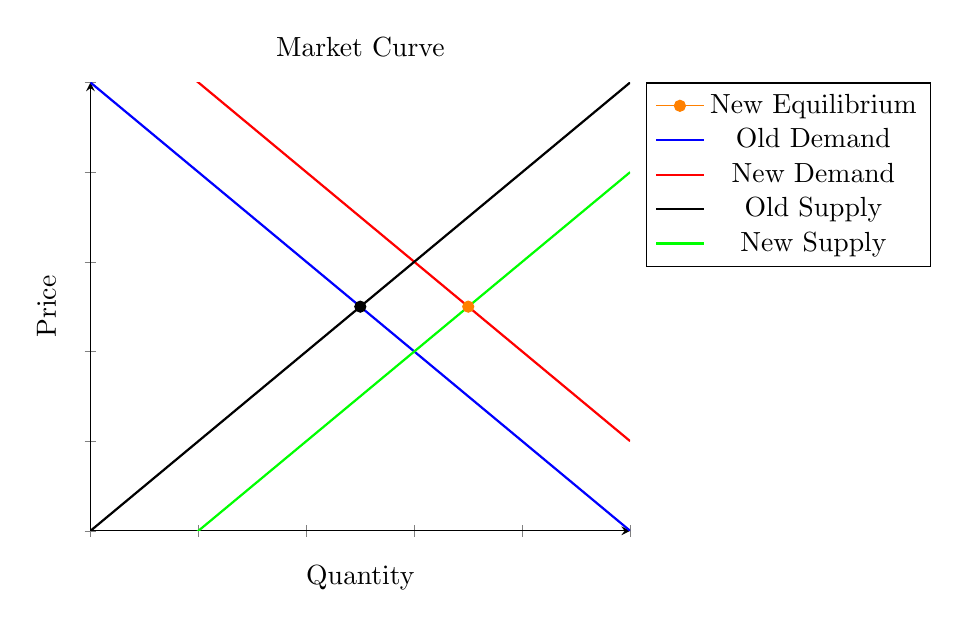
\begin{tikzpicture}
        \begin{axis}[
            title={Market Curve},
            ylabel={Price},
            xlabel={Quantity},
            yticklabel=\empty,
            xticklabel=\empty,
            xmin=0, xmax=10,
            ymin=0, ymax=10,
            axis lines=left,
            grid=none,
            legend pos=outer north east,
        ]
        

        \addplot[mark=*, color=orange] coordinates {(7,5)};
        \addlegendentry{New Equilibrium}

        \addplot[domain=0:10, color=blue, thick] {-x+10};
        \addlegendentry{Old Demand}

        \addplot[domain=0:10, color=red, thick] {-x+12};
        \addlegendentry{New Demand}

        \addplot[domain=0:10, color=black, thick] {x};
        \addlegendentry{Old Supply}

        \addplot[domain=0:10, color=green, thick] {x-2};
        \addlegendentry{New Supply}

        \addplot[mark=*] coordinates {(5,5)};
        
        \end{axis}
    \end{tikzpicture}

\end{enumerate}

\pagebreak

\question{4}

Consider the market for camp coolers. The market supply of coolersis \(Q_s = 4P\), and market demand is \(Q_d = 240 - 4P\).

\begin{enumerate}[(a)]
    \item Solve for equilibrium price and quantity in the market for camp coolers, and draw a graph illustrating this market.
    
    \begin{align*}
        4P &= 240 - 4P\\
        8P &= 240\\
        P &= 30\\
        Q &= 240 - 4(30)\\
        Q &= 120
    \end{align*}

    The equilibrium price of camp coolers is \$30, and the equilibrium quantity of camp coolers sold is 120.

    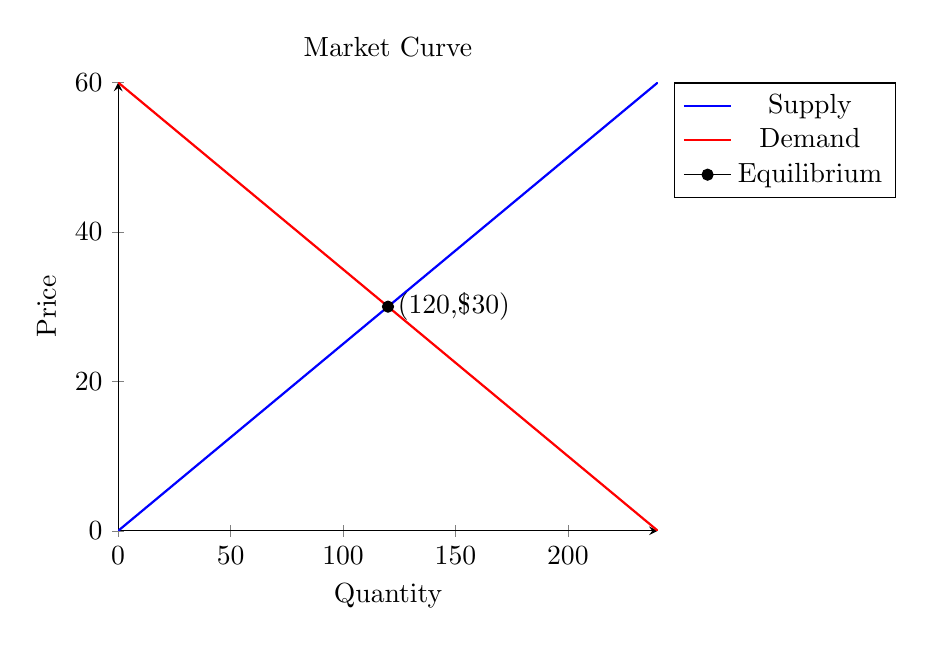
\begin{tikzpicture}
        \begin{axis}[
            title={Market Curve},
            ylabel={Price},
            xlabel={Quantity},
            xmin=0, xmax=240,
            ymin=0, ymax=60,
            axis lines=left,
            grid=none,
            legend pos=outer north east,
        ]

        \addplot[domain=0:240, color=blue, thick] {x/4};
        \addlegendentry{Supply}

        \addplot[domain=0:240, color=red, thick] {60-x/4};
        \addlegendentry{Demand}

        \addplot[mark=*, color=black] coordinates {(120,30)} node[right, pos=3] {(120,\$30)};
        \addlegendentry{Equilibrium}
        \end{axis}
    \end{tikzpicture}

    \item The government imposes a \$5 tax on those selling camp coolers. How will this change the supply function for coolers? (Hint: you may want to rearrange the supply function so that it is in the form “P=...”, like the example from our slides)
    
    \begin{align*}
        P &= \frac{Q^s}{4}\\
        P &= \frac{Q^s_{tax}}{4} + 5
    \end{align*}

    This will cause the supply function to shift to the left (up) by \$5 since the cost to produce coolers has increased by \$5.
    \pagebreak
    \item Solve for the new equilibrium price and quantity sold after the tax is implemented.
    
    \begin{align*}
        \frac{Q_{tax}}{4} + 5 &= 60 - \frac{Q_{tax}}{4}\\
        \frac{Q_{tax}}{4} + \frac{Q_{tax}}{4} &= 60 - 5\\
        \frac{Q_{tax}}{2} &= 55\\
        Q_{tax} &= 110\\
        P_{tax} &= \frac{130}{4} - 5\\
        P_{tax} &= 32.5
    \end{align*}

    The new equilibrium price of camp coolers is \$32.5, and the new equilibrium quantity of camp coolers sold is 110.

    \item Modify your graph from part (a) to show the impact of the tax.
    
    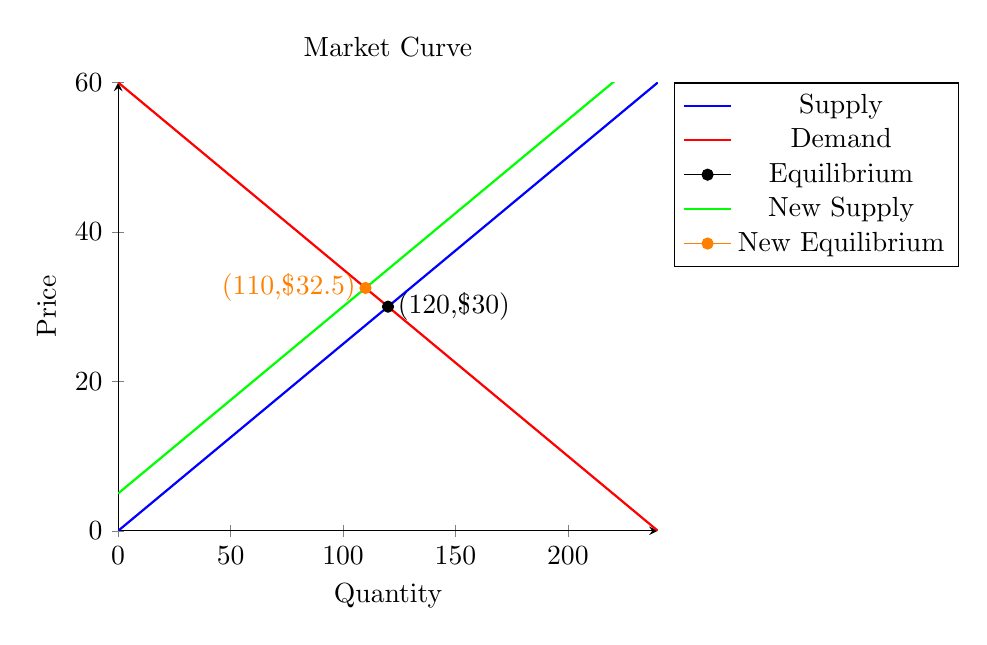
\begin{tikzpicture}
        \begin{axis}[
            title={Market Curve},
            ylabel={Price},
            xlabel={Quantity},
            xmin=0, xmax=240,
            ymin=0, ymax=60,
            axis lines=left,
            grid=none,
            legend pos=outer north east,
        ]

        \addplot[domain=0:240, color=blue, thick] {x/4};
        \addlegendentry{Supply}

        \addplot[domain=0:240, color=red, thick] {60-x/4};
        \addlegendentry{Demand}

        \addplot[mark=*, color=black] coordinates {(120,30)} node[right, pos=3] {(120,\$30)};
        \addlegendentry{Equilibrium}

        \addplot[domain=0:240, color=green, thick] {x/4 + 5};
        \addlegendentry{New Supply}

        \addplot[mark=*, color=orange] coordinates {(110,32.5)} node[left, pos=3] {(110,\$32.5)};
        \addlegendentry{New Equilibrium}
        \end{axis}

    \end{tikzpicture}
    \pagebreak
    \item Calculate how much revenue the government earns from the tax, and the deadweight loss caused by the tax.
    
    \begin{align*}
        \text{Revenue} &= \text{Tax} \times \text{Quantity}\\
        \text{Revenue} &= \$5 \times 110\\
        \text{Revenue} &= \$550
    \end{align*}
    \begin{align*}
        \text{Deadweight Loss} &= \frac{1}{2} \times \text{Tax} \times \text{Change in Quantity}\\
        \text{Deadweight Loss} &= \frac{1}{2} \times \$5 \times (120 - 110)\\
        \text{Deadweight Loss} &= \frac{1}{2} \times \$5 \times 10\\
        \text{Deadweight Loss} &= \frac{1}{2} \times \$50\\
        \text{Deadweight Loss} &= \$25
    \end{align*}

\end{enumerate}

\pagebreak

For this question, consider the market for gasoline in North Carolina. Suppose that supply and demand for gallons of gasoline can be represented with the following supply and demand functions:
\begin{align*}
    S(p) &= 30,000P\\
    D(p) &= 120,000 - 20,000P
\end{align*}

\begin{enumerate}[(a)]
    \item Use these supply and demand functions to calculate the market equilibrium for gasoline in North Carolina.
    
    \begin{align*}
        S(p) &= D(p)\\
        30,000P &= 120,000 - 20,000P\\
        50,000P &= 120,000\\
        P &= 2.4\\
        Q &= 120,000 - 20,000(2.4)\\
        Q &= 72,000
    \end{align*}

    The equilibrium price of gasoline in North Carolina is \$2.40, and the equilibrium quantity of gasoline sold is 72,000 gallons.
    
    \item Calculate producer and consumer surplus in the market for gasoline in North Carolina.

    \begin{align*}
        \text{Consumer Surplus} &= \frac{1}{2} \times 72,000 \times (6 - 2.4)\\
        \text{Consumer Surplus} &= \frac{1}{2} \times 72,000 \times 3.6\\
        \text{Consumer Surplus} &= \$129,600\\
        \text{Producer Surplus} &= \frac{1}{2} \times 72,000 \times (2.4 - 0)\\
        \text{Producer Surplus} &= \frac{1}{2} \times 72,000 \times 2.4\\
        \text{Producer Surplus} &= \$86,400
    \end{align*}

    For the rest of this question, assume also that each gallon of gasoline creates an external cost of \$0.50, due to increased healthcare costs for those individuals who breath in engine exhaust. Note that as a result, the social supply function for gasoline in North Carolina would be:

    \begin{align*}
        S_{social}(p) = 30,000p - 15,000
    \end{align*}

    \item What kind of externality is present in the market for gasoline? Will this externality cause the private market to over or underproduce gasoline?
    
    There is a negative externality present in the market for gasoline, as the social supply function is greater than the private supply function. This externality will cause the private market to overproduce gasoline.
    \pagebreak
    \item Please calculate the social optimum in North Carolina's gasoline market. Remember that, since there are no external benefits, the social demand line is equal to the private demand line.
    
    \begin{align*}
        S_{social}(p) &= D(p)\\
        30,000P - 15,000 &= 120,000 - 20,000P\\
        50,000P &= 135,000\\
        P &= 2.7\\
        Q &= 120,000 - 20,000(2.7)\\
        Q &= 66,000
    \end{align*}

    The social optimum price of gasoline in North Carolina is \$2.70, and the social optimum quantity of gasoline sold is 66,000 gallons.

    \item Draw a graph illustrating the social optimum and the private equilibrium in the market for gasoline in North Carolina. Indicate which part of your graph represents the deadweight loss caused by this externality.
    

    \begin{tikzpicture}
        \begin{axis}[
            title={Market Curve},
            ylabel={Price},
            xlabel={Quantity (in 1k gallons)},
            xmin=0, xmax=120,
            ymin=0, ymax=6,
            axis lines=left,
            grid=none,
            legend pos=outer north east,
        ]

        \addplot[domain=0:120, color=blue, thick] {x/30};
        \addlegendentry{Private Supply}

        \addplot[domain=0:120, color=red, thick] {6-x/20};
        \addlegendentry{Private Demand}

        \addplot[mark=*, color=black] coordinates {(72,2.4)} node[right, pos=3] {(72,\$2.4)};
        \addlegendentry{Equilibrium}

        \addplot[domain=0:120, color=green, thick] {x/30 + 0.5};
        \addlegendentry{Social Supply}

        \addplot[mark=*, color=orange] coordinates {(66,2.7)} node[left, pos=3] {(66,\$2.7)};
        \addlegendentry{Social Equilibrium}

        \draw[dashed, fill=red, opacity=0.5] (66,270)
            -- (72,290)
            -- (72,240)
            --cycle;
        \node[above] at (72,290) {Deadweight Loss};

        \end{axis}
    \end{tikzpicture}

    \item Now calculate the value of deadweight loss that you identified in part (e).
    
    \begin{align*}
        \text{Deadweight Loss} &= \frac{1}{2} \times (72000 - 66000) \times (0.5)\\
        \text{Deadweight Loss} &= \frac{1}{2} \times 6000 \times 0.5\\
        \text{Deadweight Loss} &= \$1500
    \end{align*}

    The value of the deadweight loss is \$1500.

    \item If the government wants to solve this externality problem the 'normal' way, would it involve using a tax or a subsidy? How large would that tax or subsidy need to be?
    
    The government would need to use a tax to solve this externality problem. The tax would need to be \$0.30, as the difference between the social optimum price and the private equilibrium price is \$0.30.

    \item What is one alternative way that the government could try to solve this externality problem? Explain in a sentence or two how your alternate solution would cause gasoline suppliers to internalize their externality.
    
    The government could also use a cap-and-trade system to solve this externality problem. This would cause gasoline suppliers to internalize their externality by allowing them to trade permits to pollute, which would allow them to find the most efficient way to reduce their pollution.

\end{enumerate}

\end{document}